%!TEX root = ../projecto.tex

\section{Introduction}

With the evolution of social networks websites like Facebook and Twitter, the amount of pertinent content about a specif issue is increasing dramatically, which calls for new ways to make sense and catalog this data.
The usage of social networks for branding quality and on-line marketing is specially compelling since 19\% of all tweets \cite{Jansen2009} and 32\% \cite{Melville2009} of blog posts are about brands or products.
In the other hand find topic sensitive information on social networks is extremely complicated due to the fact that documents have very little content, slang vocabulary and orthographically mistakes or abbreviations.

The value of data presented in sites like Facebook or Twitter as proven its value in papers like "Predicting the future with social media"  \citet{Asur2010} where it is possible to predict with high precision the value of a movie box office weeks before it debuts, through real time monitoring of the velocity of reference of Hashtags referencing debuting movies.

The academic and enterprise world is now starting to look at Machine Learning for new ways to achieve revenue and visualize data representing the way the world works. It is not strange to see that the Machine Learning course is the one with more students enrolling this year \footnote{http://www.forbes.com/sites/anthonykosner/2013/12/29/why-is-machine-learning-cs-229-the-most-popular-course-at-stanford/} with more than 760 students enrolled.

With emerging new techniques like Deep Learning \citet{Bengio2013} which focuses on abstract representations that can lead to more useful representations, one example of this kind of work is \citet{Le2011} "Building High-level Features Using Large Scale Unsupervised Learning" where a 9-layered locally connected sparse autoencoder with pooling and local contrast normalization on a large dataset of images (the model has 1 billion connections, the dataset has 10 mil- lion 200x200 pixel images downloaded from the Internet) trained using model parallelism and asynchronous SGD on a cluster with 1,000 machines (16,000 cores) during three days. Which achieved 81.7 percent accuracy in detecting human faces, 76.7 percent accuracy when identifying human body parts and 74.8 percent accuracy when identifying cats.

The application of unsupervised learning stretches to apply itself to multiple areas, such as \citet{Knight2011a} work on solving an enciphered, 105 page, from 1866 book.The document was named Copiale Cipher and was found in the East Berlin Academy after the Cold War and has been undecipherable ever since. The decifering of the document was possible due to the usage of k-means algorithm from the Scipy cluster package \footnote{http://docs.scipy.org/doc/scipy/reference/cluster.html} which is a common and simple tool for data scientists. 

While most Data Scientist are struggling to find new smarter algorithms to visualize and understand data, \citet{Halevy2009} claims that "its ll about the data" and that solutions to problems like speech recognition and automatic photo enhancements for example, can be solved by just feeding more data to the already in use algorithms. This not a new concept, actually \citet{Banko2001} at Microsoft stated a the same principle a couple o years before applied to most core natural language. One example of this principle is \citet{Hays2007a} work where he presents a new way to do scene completion where it is possible to remove elements from pictures which disappear in a way that in a lot of cases is not possible to distinguish with a naked eye.

\citet{Radinsky2013} took the next step into deep learning with predictive data-mining software by being able to predict with an accuracy of 70 to 90 percent the probability of natural disasters, disease epidemics, social unrest, and violence outbreaks. By using data gathered from Wikipedia, the 150 years of New York Times archives and web LinkedData. Her work awarded her to be in the MIT top 35 innovators under 35 \footnote{http://www.technologyreview.com/lists/innovators-under-35/2013/} and was the starting point to her own venture SalesPredict \footnote{http://www.salespredict.com/} where massive amounts of data from inside and outside the hiring company are used, in order to improve new pipeline opportunities. SalesPredict had recently raised \$1 million dollars in seed funding.

Even though a lot of solution arise in order to automate real time searches, topic categorization and many other data intensive tasks, Twitter still uses humans in order to deliver ads to trending queries, states Edwin Chen's ads quality at Twitter. On his blog post \footnote{Edwin Chen's Blog, engineer at Twitter: http://blog.echen.me/2013/01/08/improving-twitter-search-with-real-time-human-computation/} Edwin describes the process of Twitter to deliver real time adds to trending queries, the main problems that arise in the Twitter platform in order to identify rising topic are mainly:
\begin{itemize}
  \item The queries people perform have never before been seen, so it's impossible to know beforehand what they mean.
  \item Since the spikes in search queries are short-lived, there's only a short window of opportunity to learn what they mean.
\end{itemize}
This means that when an event happen, people immediately come to Twitter in order to know what is happening in a determined place in real time. Twitter solves this issue by monitoring which queries are currently popular in real time, using a Storm topology \footnote{http://storm-project.net/} and after the queries are identified, they are sent to a Thrift API that dispatches the query to Amazon's Mechanical Turk service where real people will be asked a variety of questions about the query. One example of this tweets that occur in a rather peculiar situation Jānis Krūms which tweets that he was on his way to the Hudson river to pick up people from a plane crash, the tweet is shown in figure .

\begin{figure}[tb]
  \begin{center}
    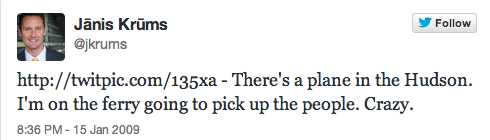
\includegraphics[width=8cm]{images/8_hudson.png}
  \end{center}
  \caption{Tweet by Jānis Krūms, while he is going to pick up some people}
  \label{fig:hudson}
\end{figure}

Social Media Analytics is another raising topic which draws from Social Network Analysis, Machine Learning, Data Mining, Information Retrieval (IR), and Natural Language Processing (NLP). As stated by \citet{Melville2009} 32\% of the 200 million bloggers world wide blog about opinions on products and brands, 71\% of the 625 million active Internet users actually read blogs and more importantly that 78\% of respondents put their trust in the opinion of other consumers where only only 57\% of consumers trust advertising in traditional media and even worst only 34\% of consumers put their trust in such advertising. This kind of data drives companies to Social Media Analytics in a way to know what people are saying on the web about their companies and products. This new worry has brought to life a lot of new startups like Sumal\footnote{https://sumall.com/} or ThoughtBuzz\footnote{http://www.thoughtbuzz.net/} but also solutions from the old players like IBM \footnote{http://www-01.ibm.com/software/analytics/solutions/customer-analytics/social-media-analytics/} and SAS \footnote{http://www.sas.com/software/customer-intelligence/social-media-analytics.html}

Its also important to notice that in the last few years Data Science/Analysis has been a trended topic, mostly due to the fact that big dot-com companies have been making lots of money through exploiting user specific information in order to deliver ads and sell products. No wonder that if you look that in the top 10 ebooks sold by O'Reilly throuout 2013 four are about data science \footnote{http://shop.oreilly.com/category/deals/best\-of\-oreilly\-dotd.do?code=DEAL\&cmp=tw\-na\-books\-videos\-info\-authornote\_best\_of\_2013}.

In this project we will focus on using an unsupervised learning technique based on neural networks named Self-organizing Map \cite{Kohonen1990} in order to detect topics in Twitter posts, by using the Social Network users as base neurons for clustering. After the network is trained it will be possible to categorize tweets in real time. This approach will be better described in subsection \ref{sub:objectives}.

First this report will be dedicated to explain some basics concepts like Document CLustering and specifically Self-organizing Maps in section \ref{sec:basic_concepts}.  Further in, section \ref{sec:related_work} will be dedicated to the state of the art solutions related not only to topic detection but also to twitter data analysis and Self-Organizing Maps.In section \ref{sec:architecture} Architecture of the purposed solution and  at section \ref{sec:evaluation_metrics} it will be discussed how to evaluate results achieved. Finally we will this report by referencing some possible future work and with a brief conclusion at section \ref{sec:coclusions_future_work}.

\subsection{Objectives} % (fold)
\label{sub:objectives}

The objective of this project is clear, finding topics on Tweets by analyzing their corpus specific characteristics, like number of characters in a tweet, Hashtag, “was retweeted”, etc.. And contextualize the social network evolving the person that did the tweet.

After characterizing the tweet with information just described, we will use the unsupervised learning clustering technique Self-organizing maps in order to organize the tweets in clusters of topics. Afterwards it will be needed to categorize the clusters in order to know which topic they belong to.

Lastly the resulting topic clusters will be publicly accessible through a website to everybody that visits it.
% section objectives (end)
% subsection objectives (end)
